\chapter{Estudio Administrativo Legal}

\section{Filosofía de la empresa}

\subsection{Misión}


Ofrecer soluciones innovadoras y sostenibles para el cultivo de plantas en entornos controlados. Nos especializamos en el diseño y fabricación de cabinas de alta calidad que optimizan el cuidado de las plantas al proporcionar condiciones ideales de luz, temperatura y humedad.



\subsection{Visión}

Nos visualizamos como líderes en la industria de cabinas para el cuidado de plantas, contribuyendo tanto al bienestar de las personas como al cuidado del medio ambiente. Ser reconocidos por nuestra excelencia en diseño, tecnología y nuestro firme compromiso con la sustentabilidad.


\subsection{Valores de la empresa}

\begin{itemize}

 \item \textbf{Innovación:} Estamos en busca de nuevas maneras de mejorar nuestras cabinas y procesos.
    \item \textbf{Calidad:} Nos dedicamos a ofrecer productos que sean duraderos y confiables.
    \item \textbf{Sostenibilidad:} Prestamos atención al impacto ambiental en cada etapa de producción.
    \item \textbf{Colaboración:} Trabajamos codo a codo con nuestros clientes y socios para alcanzar resultados excepcionales.

\end{itemize}

\subsection{Politicas de la empresa}


\begin{itemize}
    \item \textbf{Compromiso con la Sostenibilidad:} Nos comprometemos a diseñar y fabricar nuestras cabinas de manera sostenible, utilizando materiales y procesos de producción eficientes. Buscamos reducir nuestra huella de carbono y minimizar el impacto ambiental en cada etapa de la cadena de suministro.
    
    \item \textbf{Calidad y Durabilidad:} Nuestro objetivo es ofrecer productos de alta calidad y duraderos. Todas nuestras cabinas están diseñadas para resistir el paso del tiempo y brindar un servicio confiable a nuestros clientes.
    
    \item \textbf{Atención al Cliente:} Valoramos a nuestros clientes y nos esforzamos por brindar un excelente servicio. Estamos disponibles para resolver dudas, ofrecer asesoramiento y garantizar la satisfacción del cliente.
    
    \item \textbf{Innovación y Mejora Continua:} Fomentamos la innovación en nuestros diseños y procesos. Buscamos constantemente nuevas formas de mejorar nuestras cabinas para satisfacer las necesidades cambiantes del mercado.
    
    \item \textbf{Colaboración y Trabajo en Equipo:} Trabajamos en estrecha colaboración con nuestros clientes, proveedores y socios para lograr resultados excepcionales. Valoramos la diversidad de ideas y creemos en el poder del trabajo en equipo.
    
    \item \textbf{Ética y Responsabilidad Social:} Cumplimos con todas las regulaciones y normativas aplicables. Contribuimos positivamente a la comunidad y al medio ambiente a través de acciones responsables y programas de responsabilidad social.
\end{itemize}


\section{Análisis FODA de la empresa}

\subsection{Fortalezas}

\begin{itemize}
    \item Producto innovador y único en el mercado.
    \item Ahorro de tiempo para los clientes al automatizar el cuidado de las plantas.
    \item Posibilidad de personalización según las necesidades de los usuarios.
    \item Enfoque ecológico y sostenible.
    \item Fuerte presencia en línea, facilitando el acceso y la compra para los clientes.
    \item Equipo altamente calificado y comprometido con la excelencia en el servicio al cliente.
    \item Estrategias de marketing efectivas que destacan las ventajas competitivas del producto.
    \item Capacidad de adaptación rápida a las tendencias del mercado y a las necesidades de los clientes.
    \item Red de distribución establecida que permite llegar a una amplia audiencia de manera eficiente.

\end{itemize}

\subsection{Oportunidades}

\begin{itemize}
    \item Interés creciente en la jardinería interior y el bienestar.
    \item Alianzas con viveros y centros de jardinería para promover las cabinas.
    \item Expansión internacional a nuevos mercados emergentes con alta demanda de productos de jardinería.
    \item Colaboración con empresas de tecnología para desarrollar nuevas funcionalidades y mejoras en el producto.
    \item Aprovechamiento de programas de incentivos gubernamentales para empresas que promueven la sostenibilidad.
    \item Desarrollo de aplicaciones móviles y plataformas en línea para ofrecer servicios adicionales a los clientes.
    \item Participación en ferias y eventos de jardinería para aumentar la visibilidad de la marca y generar clientes potenciales.
    \item Ofrecimiento de programas de financiamiento o leasing para facilitar la adquisición de las cabinas a los clientes.
    \item Diversificación del portafolio de productos para incluir accesorios y complementos relacionados con el cuidado de las plantas.

    \item Expansión a espacios comerciales como oficinas, hoteles y restaurantes.
    \item Integración con sistemas domóticos y tecnología IoT.
    
\end{itemize}

\subsection{Debilidades}

\begin{itemize}
    \item Competencia de otros productos y servicios de cuidado de plantas.
    \item Crisis económicas que afecten el gasto del consumidor.
    \item Desafíos regulatorios y cumplimiento de normativas.
    \item Dependencia de proveedores clave para componentes específicos de las cabinas, lo que podría afectar la disponibilidad y los costos.
    \item Limitaciones en la capacidad de producción que podrían dificultar la satisfacción de la demanda en momentos de alta temporada.

    
    
\end{itemize}

\subsection{Amenazas}

\begin{itemize}
    \item Costo inicial elevado para fabricar y adquirir las cabinas.
    \item Necesidad de educar al mercado sobre los beneficios de la automatización.
    \item Mantenimiento y actualización de software pueden ser complejos.
    \item Dependencia de la tecnología y posibles fallas.
\end{itemize}

\section{Estructura organizacional de la empresa}

La estructura organizacional es fundamental para el éxito financiero de una empresa. Al definir roles y responsabilidades, se logra una gestión financiera eficiente, rendición de cuentas, toma de decisiones ágil y mitigación de riesgos.

Una estructura organizacional bien diseñada permite asignar tareas de manera efectiva al definir claramente las funciones y responsabilidades de cada empleado. Al definir roles y responsabilidades, la estructura organizacional mejora la responsabilidad dentro de la empresa. Además, una estructura organizacional sólida ayuda a minimizar riesgos. Al definir roles y responsabilidades, se establecen límites claros, lo que reduce la posibilidad de conflictos y malentendidos.

\subsection{Organigrama}

Como correcciones del primer organigrama preliminar, se propone ahorrar gastos de salario contratando solo a los ingenieros necesarios a cambio de mayor mano de obra. Quedando así el cronograma.

\begin{figure}[H]
    \centering	
    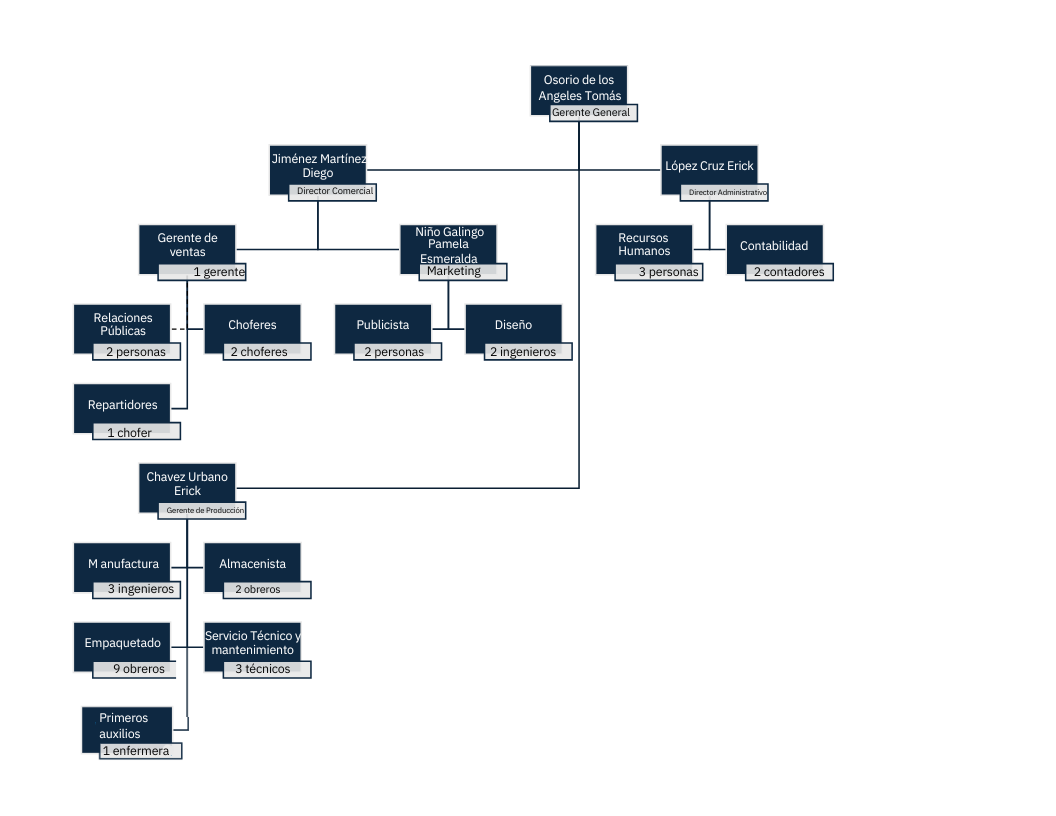
\includegraphics[width=1.3\textwidth]{img/Empresa/ORGANIGRAMA.png} 
    \caption{Se propone contratar menos ingenieros y más obreros o técnicos.}
\label{fig:macrolocalizacion}
\end{figure}

Además, se añadió un empleado destinado para primeros auxilios en el área de producción.
\newpage

\subsection{Descripción de funciones por área de operación}
\textbf{Personal administrativo}

\begin{longtable}[p]{ |p{2cm}||p{2cm}|p{4.5cm}|p{4.5cm}| }

 \hline
 Nombre del puesto & Jefe inmediato & Escolaridad & Descripción de funciones\\
 \hline
 \endfirsthead

 \hline
 Nombre del puesto & Jefe inmediato & Escolaridad & Descripción de funciones\\
 \hline
 \endhead
 
 \hline
 Director Comercial & Gerente General & Lic. en Adminstración de Empresas o área relacionada \newline Mtro. en Administrador de negocios (Deseable) &  Desarrollar y ejecutar estrategias comerciales para alcanzar los objetivos de ventas y crecimiento de la empresa.\\
 \hline
 Gerente de Ventas & Gerente General  & Lic. en Adminstración de Empresas o área relacionada &  Supervisar y capacitar al equipo de ventas, estableciendo
metas y evaluando el desempeño\newline Identificar oportunidades de crecimiento en
el mercado y desarrollar relaciones con clientes clave.\\
 \hline
 Gerente de Marketing & Gerente General & Lic. en Marketing, Comunicación, Administración de Empresas o carrera afín & Coordinar campañas
publicitarias, eventos promocionales y actividades de relaciones públicas.\\
 \hline
 Gerente de Recursos Humanos & Gerente General & Lic. en Administración de Empresas, Psicología Organizacional, Recursos Humanos o carrera afín & Gestionar el clima laboral y las relaciones
laborales, promoviendo un ambiente de trabajo positivo y colaborativo.\\
 \hline
 Gerente de Producción & Gerente General & Ing. Industrial, Mecatrónica o carrera afín & Desarrollar e implementar estrategias de mejora continua para incrementar la eficiencia operativa y la rentabilidad\\
 \hline
 
 \end{longtable}
 \newpage

\textbf{Personal de producción}

\begin{longtable}[p]{ |p{2cm}||p{2cm}|p{4.5cm}|p{4.5cm}| }

 \hline
 Nombre del puesto & Jefe inmediato & Escolaridad & Descripción de funciones\\
 \hline
 \endfirsthead

 \hline
 Nombre del puesto & Jefe inmediato & Escolaridad & Descripción de funciones\\
 \hline
 \endhead
 
 \hline
Obrero de producción\newline Técnico de producción & Gerente de Producción & Educación bachiller completa\newline Certificados de formación en áreas específicas de producción (deseable) & Operar maquinaria y equipos según los procedimientos establecidos\newline Realizar tareas manuales, como ensamblaje, empaque o carga y descarga de materiales\\
 \hline
 Repartidor\newline Chofer & Gerente de Producción &  Licencia de conducir vigente y categoría adecuada para vehículos de 2 toneladas & Conducir vehículos de reparto o transporte según las rutas establecidas y los horarios asignados\newline Cargar y descargar mercancías de manera segura y
 eficiente\newline Mantener el vehículo limpio y en buen estado de funcionamiento\\
 \hline
 Primeros Auxilios & Gerente de Producción &  Certificación en primeros auxilios\newline Lic. en Enfermería (Deseable) & Estar atento al estado de salud de los trabajadores en el área de producción\newline Proporcionar asistencia inmediata para lesiones menores, como cortes, raspaduras o quemaduras leves\newline Asegurarse de que el botiquín esté bien abastecido y en un lugar accesible\\
 \hline
\end{longtable}
\newpage

\textbf{Personal de mercadotecnia y ventas}

\begin{longtable}[p]{ |p{2cm}||p{2cm}|p{4.5cm}|p{4.5cm}| }

 \hline
 Nombre del puesto & Jefe inmediato & Escolaridad & Descripción de funciones\\
 \hline
 \endfirsthead

 \hline
 Nombre del puesto & Jefe inmediato & Escolaridad & Descripción de funciones\\
 \hline
 \endhead
 
 \hline

 Contador & Director Administrativo &  Lic. en Contaduría Pública, Administración de Empresas o carrera afín & Registrar y verificar en el sistema los movimientos y transacciones contables realizadas en la empresa\newline Revisar y señalar las variaciones encontradas con respecto a períodos anteriores\newline Registrar y balancear las entradas contables y las transacciones de intercambio semanal de pago a los bancos, relacionadas al Departamento de Servicios Internacionales\\
 \hline

\end{longtable}
\newpage

\subsection{Administración de personal}

\textbf{Planeación}

Para proyectar el crecimiento del personal, utilizamos el mismo porcentaje de crecimiento obtenido en la sección \textbf{Proyección de la Demanda}. en nuestro caso, utilizamos la fórmula aplicada a los valores existentes y obtenemos \[ Empleados = 33 + 2.7489x\]

\begin{tabular}{ |p{1cm}|p{2cm}|p{3cm}|p{3cm}|p{3cm}|  }
 \hline
 \multicolumn{5}{|c|}{PERSONAL\newline (Número de empleados)} \\
 \hline
 Año & Producción & Administración & Mercadotecnia y Ventas & Total de empleados\\
 \hline
 1 & 18 & 5 & 10 & 33\\
 \hline
 2 & 20 & 5 & 11 & 36\\
 \hline
 3 & 22 & 6 & 12 & 40\\
 \hline
 4 & 24 & 6 & 13 & 43\\
 \hline
 5 & 26 & 7 & 14 & 47\\
 \hline
 6 & 28 & 7 & 15 & 50\\
 \hline
\end{tabular}

\textbf{Reclutamiento}

El reclutamiento se hará de conocimiento a la población por medio de radio difusión, anuncios en puntos clave de la ciudad al igual que pancartas.

Como documentación general se solicitarán los siguientes documentos.

\begin{enumerate}
    \item Acta de Nacimiento
    \item CURP
    \item Número de Seguridad Social (NSS)
    \item Comprobante de Domicilio
    \item CV
    \item Certificados y Diplomas
    \item Cartas de Recomendación
\end{enumerate}

\textbf{Selección}

El personal de Recursos Humanos serán los encargados de realizar el proceso de selección en todo momento. A los aspirantes a puestos administrativos se le deberá realizar un examen de habilidades acorde a su área y estando relacionadas con las futuras actividades a realizar.

\begin{itemize}
    \item ¿Qué aspectos crees que te diferencian como ingeniero?
    \item ¿Cómo manejas situaciones de presión o crisis en un proyecto?
    \item ¿Qué producto crees que se comercializa mal?
    \item ¿Cuál es la última campaña de marketing que te llamó la atención?
    \item ¿Cuántos años de experiencia tienes como contador?
    \item ¿En qué áreas de la contabilidad te especializas?
    \item ¿Qué software contable has utilizado en tus trabajos anteriores?
\end{itemize}

\textbf{Contratación}

Primero se ofrecerá un contrato por un mes, dependiendo del desempeño se ofrecería posteriormente uno de 3 meses y finalmente un contrato indefinido. El puesto del empleado dependerá de su desempeño.

\textbf{Inducción}

Para el curso de inducción se ocupará medio día laboral completo, donde se le mostrará a los nuevos empleados las instalaciones de trabajo, medidas y procesos de seguridad, una breve introducción a su trabajo para finalmente asignarle el nuevo trabajador al encargado del área.

\textbf{Capacitación}

Al momento del arranque de operaciones, el personal administrativo será el primero en recibir la capacitación necesaria para procesos de manufactura, posteriormente se le impartirán estos cursos al personal restante dependiendo del cambio de empleados.

%%%%%%%%%%%%%%%%%%%%%%%%%%%%%%%%%%%%%%%
\section{Conclusiones del estudio administrativo}

La empresa tiene una misión y visión claramente definidas, enfocadas en la innovación, sostenibilidad y calidad. Sus valores fundamentales, como la innovación, calidad, sostenibilidad y colaboración, orientan todas sus actividades y decisiones estratégicas. Esta alineación entre misión, visión y valores asegura que la empresa mantenga un enfoque coherente en su desarrollo y crecimiento.

La estructura organizacional está bien definida, con roles y responsabilidades claramente asignados. Esto contribuye a una gestión financiera eficiente y a la minimización de riesgos. La propuesta de reducir el número de ingenieros y aumentar la mano de obra puede ser una estrategia eficaz para optimizar costos y mejorar la eficiencia operativa.

Las descripciones detalladas de los puestos aseguran que cada empleado conozca sus responsabilidades y objetivos. Esto es vital para el buen funcionamiento de la empresa y para mantener un ambiente laboral positivo y productivo. La planificación del crecimiento del personal, basada en la proyección de la demanda, muestra una estrategia proactiva para manejar el aumento de la carga de trabajo a medida que la empresa crece.

El estudio muestra que nuestra   empresa está bien posicionada para alcanzar sus objetivos de liderazgo en el mercado de cabinas para el cuidado de plantas. La clara definición de su filosofía, una estructura organizacional robusta y una planificación cuidadosa del personal son elementos clave para su éxito. Es fundamental que la empresa continúe monitoreando y ajustando sus estrategias según las dinámicas del mercado y las necesidades internas para mantener su competitividad y sostenibilidad a largo plazo.


\section{Marco jurídico para la puesta en marcha}


\subsection{Figura jurídica de la empresa}
La figura jurídica elegida para nuestra empresa, que se dedicará a la fabricación de cabinas climáticas para plantas, es la Sociedad de Responsabilidad Limitada (S. de R.L.). Esta decisión se basó en las ventajas que ofrece este tipo de sociedad, tales como la limitación de la responsabilidad de los socios al monto de sus aportaciones, la flexibilidad en la gestión y el capital inicial accesible.
\subsection{Requisitos para la constitución de la empresa}
Para constituir una Sociedad de Responsabilidad Limitada en México, se deben seguir los siguientes pasos:
\textbf{Autorización del nombre comercial:}
Obtener la autorización de la Secretaría de Economía para el uso del nombre comercial de la empresa, asegurando que no exista otra empresa con el mismo nombre. Este trámite se puede realizar en línea utilizando la e.firma.

\textbf{Elaboración del acta constitutiva:}
Con la asistencia de un notario, se debe elaborar el acta constitutiva de la empresa. Este documento establece los aspectos legales generales y particulares de la empresa, incluyendo el objeto social, capital social y normas de funcionamiento. Todos los socios deben firmar el acta.

\textbf{Aviso de uso de denominación:}
El funcionario que llevó a cabo la constitución de la sociedad debe informar a la Secretaría de Economía sobre las personas que se han asociado para crear la nueva empresa y el nombre que usarán, para evitar su uso por otras personas ajenas a la sociedad.

\textbf{Registro público de comercio:}
Inscribir la empresa en el Registro Público de Comercio, entidad que supervisa y protege a las empresas. Este trámite requiere el pago de derechos de inscripción, cuyo costo varía según el estado y el cual se especificará mas adelante \ref{sec:permisos}.

\textbf{Registro Federal de Contribuyentes (RFC):}
Realizar el trámite ante el Servicio de Administración Tributaria (SAT) para identificar la empresa como persona moral.

\textbf{Registro ante el IMSS:}
Registrarse en el Instituto Mexicano del Seguro Social (IMSS), incluso si los únicos trabajadores iniciales son los socios fundadores. No cumplir con este requisito puede resultar en multas.

\textbf{Inscripción en organismos adicionales:}
Inscribirse en otras instituciones según el tipo de actividad de la empresa, el municipio y el estado en el que se ubique. Esto puede incluir la Secretaría de Ecología y Medio Ambiente o el Instituto Mexicano de la Propiedad Intelectual, entre otros.

%Trámites de Licencia Municipal:
%a) Obtener la licencia municipal para la construcción de obra civil.
%b) Obtener la licencia municipal para el funcionamiento de la empresa, conforme a los reglamentos vigentes del municipio donde se establecerá la empresa.

\subsection{Elementos de un acta constitutiva}
El acta constitutiva es el documento obligatorio que da constancia y legalidad a la constitución de una sociedad al momento de crear una empresa. Este documento debe incluir los siguientes elementos:

\textbf{Datos de los constituyentes:}
Nombres, nacionalidad y domicilio de las personas físicas o morales que constituyen la sociedad.

\begin{itemize}
    \item Erick Chávez Urbano, Mexicana, Union y Progreso \#10 Cuilapam de Guerrero Oaxaca.
    \item Diego Jiménez Martínez, Mexicana, Privada de independencia \#26 Magdalena Etla.
    \item Pamela Esmeralda Galindo Niño, Mexicana, Privada de independencia \#40 Etla.
    \item Tomás Osorio de los Ángeles, Mexicana, Benito Juárez \#30, Acatlima Huajuapan.
    \item Erick López Cruz, Mexicana, Av. Modesto Seara Vásquez \#19
\end{itemize}

\textbf{Objeto social}
Descripción del objeto de la sociedad.

La sociedad tiene por objeto la realización de las siguientes actividades:
\begin{itemize}
    \item \textbf{Diseño, fabricación y comercialización de cabinas climáticas:} Diseñar, desarrollar, fabricar y comercializar cabinas climáticas para plantas, adecuadas para su uso en oficinas, hogares y cualquier otro espacio cerrado.
    \item \textbf{Instalación y mantenimiento de equipos:} Proveer servicios de instalación, mantenimiento preventivo y correctivo, así como la reparación de cabinas climáticas y otros sistemas relacionados con el control ambiental para plantas.
    \item \textbf{Investigación y desarrollo:} Realizar investigaciones y desarrollar nuevas tecnologías y métodos relacionados con el control climático, automatización y optimización del crecimiento de plantas en ambientes controlados.
    \item \textbf{Venta de accesorios y componentes:} Comercializar accesorios, componentes y repuestos necesarios para el funcionamiento y mantenimiento de las cabinas climáticas.
    \item \textbf{Capacitación y asesoría:} Ofrecer servicios de capacitación, asesoría técnica y consultoría a empresas, instituciones y particulares en relación con el uso, instalación y mantenimiento de las cabinas climáticas y otros sistemas de control ambiental.
    \item \textbf{Desarrollo de software y soluciones tecnológicas:} Desarrollar y comercializar software y soluciones tecnológicas que mejoren la eficiencia y funcionalidad de las cabinas climáticas, incluyendo sistemas de monitoreo y control remoto.
    \item \textbf{Importación y exportación:} Importar y exportar productos, materiales, equipos y tecnologías relacionados con las cabinas climáticas y el control ambiental para plantas.
    \item \textbf{Participación en proyectos y licitaciones:} Participar en proyectos, concursos, licitaciones y cualquier tipo de contratación pública o privada relacionada con la fabricación, instalación y mantenimiento de cabinas climáticas y sistemas de control ambiental.
\end{itemize}

\textbf{Razón social o denominación:}
El nombre bajo el cual operará la sociedad.
Nombre de la empresa: TerraGreen.

\textbf{Duración:}
Indefinido.

\textbf{Capital social:}
El importe del capital social, incluyendo las aportaciones de cada socio, ya sea en dinero o en otros bienes, y el criterio seguido para su valorización. Si el capital es variable, se debe indicar el mínimo establecido.

\begin{itemize}
    \item Erick Ch. -> \$ 5000
    \item Diego -> \$ 5000
    \item Esmeralda G. -> \$ 5000
    \item Tomás O. -> \$ 5000
    \item Erick Lo. -> \$ 5000
\end{itemize}

\textbf{Domicilio:}
El domicilio de la sociedad.

Colonia el Tepeyac, Juan Diego \#19, esquina con Díaz Ordaz, Huajuapan de león, Oaxaca, México.

\textbf{Administración:}
La manera en que se administrará la sociedad y las facultades de los administradores.

\textbf{Nombramiento de administradores:}
La designación de los administradores y los responsables de llevar la firma social.

\textbf{Distribución de utilidades y pérdidas:}
La manera de distribuir las utilidades y pérdidas entre los socios.

\textbf{Fondo de reserva:}
El importe del fondo de reserva es del 15\% de las ganancias anuales.

\textbf{Disolución anticipada:}
Los casos en que la sociedad puede disolverse anticipadamente.

\textbf{Liquidación:}
Las bases para la liquidación de la sociedad y el procedimiento para elegir a los liquidadores, si no fueron designados anticipadamente.

\subsection{Permisos municipales}
\label{sec:permisos}
\textbf{Licencia para construcción de una obra}
Los requisitos del municipio de Huajuapan de león pueden verse en el siguiente anexo \ref{sec:requisitosMunicipales}

El costo por permisos de construcción dependerán del tamaño de la obra y del municipio, varía entre un mínimo de \$471 y un máximo de \$7426 MXN. \cite{permisos2024Mexico}

\textbf{Licencia para el funcionamiento de la empresa}
A continuación se listan los documentos necesarios:
\begin{itemize}
    \item Acta constitutiva, original y 2 copias.
    \item Identificación oficial, original y 2 copias.
    \item RFC, original y 2 copias.
    \item Comprobante de domicilio, original y 2 copias.
    \item Croquis de ubicación, original y 2 copias.
    \item Comprobante de pago, original y 2 copias.
\end{itemize}

El pago correspondiente para este tipo de licencias varía según el municipio pero según el gobierno de méxico este monto corresponde a una cantidad de: \$ 3,211.00 MXN \cite{Licencia2024Mexico}


%\subsubsection{Licencia para la construcción de una obra civil}
%\subsubsection{Licencia para el funcionamiento de la empresa}

\section{Marco jurídico bajo el cual se regirán las operaciones de la empresa}

\subsection{ Normas Oficiales Mexicanas (NOMs)}

\textbf{Normas de Seguridad y Salud en el Trabajo}

NOM-001-STPS-2008: Edificios, locales, instalaciones y áreas en los centros de trabajo - Condiciones de seguridad.
Establece las condiciones de seguridad en las instalaciones laborales, que incluyen la infraestructura donde se encuentran las cámaras climáticas.

NOM-002-STPS-2010: Condiciones de seguridad - Prevención y protección contra incendios en los centros de trabajo.
Especifica las medidas para la prevención y protección contra incendios, relevante para la seguridad de las instalaciones.

NOM-022-STPS-2015: Electricidad estática en los centros de trabajo - Condiciones de seguridad.

\textbf{Normas Ambientales}

NOM-081-SEMARNAT-1994: Establece los límites máximos permisibles de emisión de ruido de las fuentes fijas y su método de medición.

Aplica si las cámaras climáticas generan ruido, asegurando que no excedan los límites permitidos.
NOM-085-SEMARNAT-2011: Contaminación atmosférica - Control de emisiones de fuentes fijas.

Regula las emisiones atmosféricas de fuentes fijas, pertinente si las cámaras climáticas utilizan sistemas que emiten contaminantes.

\textbf{Seguridad relacionadas con la electricidad estática}

Para cámaras climáticas, es posible que deban cumplirse varias NOMs dependiendo de sus características específicas, como:

NOM-024-SCFI-2013: Información comercial para empaques, instructivos y garantías de los productos electrónicos, eléctricos y electrodomésticos.

NOM-003-SCFI-2014: Productos eléctricos - Especificaciones de seguridad.

Recomendaciones
Revisión de Etiquetado y Publicidad: Asegurarse de que toda la información proporcionada sobre las cámaras climáticas sea veraz y suficiente.
Implementación de Garantías: Ofrecer garantías claras y cumplir con ellas de manera efectiva.
Atención al Cliente: Establecer un sistema eficiente para manejar quejas y reclamaciones.
Cumplimiento de NOMs: Identificar y cumplir con todas las NOMs aplicables a los productos.
Cumplir con la LFPC y las NOMs no solo es una obligación legal, sino que también contribuye a la confianza y satisfacción del consumidor, lo cual es vital para el éxito comercial de la empresa.

\textbf{Normas de Equipos y Productos}

NOM-003-SCFI-2014: Productos eléctricos - Especificaciones de seguridad.

Establece las especificaciones de seguridad para productos eléctricos, aplicable a los componentes eléctricos de las cámaras climáticas.

NOM-016-ENER-2016: Eficiencia energética de equipos y aparatos eléctricos - Límites, métodos de prueba y etiquetado.

Define los requisitos de eficiencia energética para equipos eléctricos, relevante para las cámaras climáticas que operan continuamente.



\subsection{Código de Comercio}

El contrato está regulado en los artículos 371 al 382 del Código de Comercio.

Definición y Alcance: El Código de Comercio regula los actos de comercio, las obligaciones de los comerciantes y las relaciones contractuales derivadas de estos actos. En este contexto, la fabricación y venta de cámaras climáticas se consideran actos de comercio.

Contratos Comerciales:

Compraventa Mercantil: El contrato de compraventa es uno de los más relevantes para la empresa fabricante de cámaras climáticas.  Define los derechos y obligaciones de las partes en una transacción comercial.

Contratos de Distribución y Agencia: También pueden ser relevantes para la comercialización de las cámaras climáticas. Aunque estos contratos no están específicamente definidos en el Código de Comercio, se regulan bajo las disposiciones generales de los contratos mercantiles.




 \subsection{Ley Federal de Protección al Consumidor (LFPC)}

La LFPC establece derechos y obligaciones tanto para los consumidores como para los proveedores de bienes y servicios, garantizando que los consumidores reciban productos y servicios de calidad, con información clara y veraz, y con la posibilidad de hacer valer sus derechos en caso de incumplimientos o abusos por parte de los proveedores.

Algunos puntos clave de la LFPC que pueden ser relevantes para la fabricación y comercialización de cámaras climáticas para flores incluyen:

Información y Publicidad: La ley exige que toda la información proporcionada sobre el producto sea clara, veraz y suficiente, evitando cualquier tipo de publicidad engañosa.

Garantías: Debes ofrecer garantías mínimas sobre la calidad y funcionalidad del producto.

Seguridad: Asegurar que los productos no representen un riesgo para la salud o seguridad de los consumidores.

Reclamaciones y Devoluciones: Establece procedimientos para que los consumidores puedan presentar quejas o reclamaciones y obtener compensaciones o devoluciones en caso de productos defectuosos o incumplimientos en las condiciones ofrecidas.

\section{Conclusiones del marco jurídico}

El marco jurídico establecido para la puesta en marcha de la empresa es sólido y bien fundamentado, asegurando que todas las bases legales necesarias estén cubiertas para iniciar operaciones con éxito.

La elección de la figura jurídica de Sociedad de Responsabilidad Limitada (S. de R.L.) es acertada, ya que ofrece ventajas significativas como la limitación de la responsabilidad de los socios al monto de sus aportaciones, flexibilidad en la gestión y un capital inicial accesible. Esto proporciona una estructura legal que protege a los socios y facilita la administración de la empresa.

El proceso detallado para la constitución de la empresa, que incluye desde la autorización del nombre comercial hasta la inscripción en el Registro Federal de Contribuyentes (RFC) y el Instituto Mexicano del Seguro Social (IMSS), asegura que la empresa cumpla con todos los requisitos legales y administrativos. Este enfoque meticuloso minimiza riesgos y garantiza el cumplimiento de las normativas vigentes.

El acta constitutiva, que incluye datos de los socios, el objeto social, la razón social, la duración de la sociedad, el capital social, el domicilio y la administración, establece una base legal clara y detallada para la operación de la empresa. La inclusión de todos estos elementos asegura que la empresa esté bien fundamentada y que los roles y responsabilidades de los socios y administradores estén claramente definidos. La obtención de permisos municipales necesarios para la construcción de una obra civil y el funcionamiento de la empresa demuestra un compromiso con el cumplimiento de las normativas locales, lo cual es crucial para la operación legal y ordenada de la empresa.

Finalmente, el marco jurídico bajo el cual se regirán las operaciones de la empresa, basado en el Código de Comercio, proporciona una estructura clara para la regulación de los actos de comercio, las obligaciones de los comerciantes y las relaciones contractuales. Los contratos comerciales específicos, como la compraventa mercantil y los contratos de distribución y agencia, están bien definidos, lo que facilita las transacciones comerciales y asegura que las relaciones con los clientes y distribuidores se manejen de manera legal y eficiente.